\chapter{Appendix A}\label{sec:appendix a}
    \begin{figure}[h]
        \centering
        \includesvg[width=.8\textwidth]{drawings/sample_stage_-_exploded}%
        \caption[Sample stage exploded view.]{Sample stage exploded view.}%
        \label{fig:sample stage exploded}%
    \end{figure}
    \newpage
    % ===================================================================================
    \begin{figure}[h]
        \centering
        \includesvg[width=.8\textwidth]{drawings/sample_drive_dimetric.svg}%
        \caption[Sample drive.]{Sample drive.}%
        \label{fig:sample drive}%
    \end{figure}
    \newpage
    % ===================================================================================
    \begin{figure}[h]
        \centering
        \includegraphics[width=\textwidth]{pictures/footage/non_boxed_full_build.png}
        \caption[Photograph of the full assembly]{Photograph of the full assembly. Fused, filtered and switchable mains voltage plug (1), Raspberry Pi 4 B (2), BigTreeTech Octopus 1.1 with 2 x TMC2209 stepper drivers (3), \qty{24}{\volt} \qty{150}{\watt} PSU (4), \qty{5}{\volt} \qty{25}{\watt} PSU (5), XRS (6), detector stage drive (7), sample stage drive (8), detector unit (9), detector and sample stages (10).}%
        \label{fig:non boxed full assembly}
    \end{figure}
    \newpage
    % ===================================================================================
    \begin{figure}[h]
        \centering
        \includesvg[height=.92\textheight]{electronics/pdf/peripherals}
        \caption[Schematics of all electronic peripherals]{Schematics of all electronic peripherals.}%
        \label{fig:schematics of peripherals}
    \end{figure}
    \newpage
    % ===================================================================================
    \begin{figure}[h]
        \centering
        \includesvg[width=.9\textwidth]{electronics/sim/LT1009}
        \caption[Simulation of the trim-resistor value dependent behavior of the \textit{LT1009} voltage reference]{Simulation of the trim-resistor value dependent behavior of the \textit{LT1009} voltage reference. At \(R_2 \approx 0\) the value output voltage is \(\approx \qty{2.385}{\volt}\).}%
        \label{fig:LT1009 sim}
    \end{figure}
    \newpage
    % ===================================================================================
    \begin{figure}
        \centering
        \begin{subfigure}{.3\textwidth}
            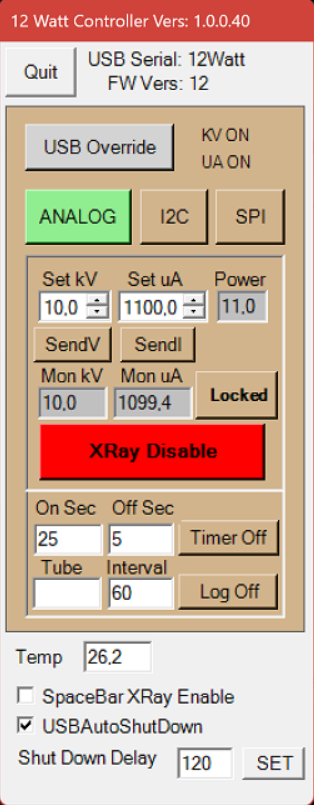
\includegraphics[width=\textwidth]{pictures/12WattController_10kV_1100uA.png}
            \caption[Set point of \qty{10}{kV} and \qty{1100}{\micro\ampere}]{Set point of \qty{10}{kV} and \qty{1100}{\micro\ampere}.}%
            \label{subfig:12WattController 10kV}
        \end{subfigure}
        \hspace{10mm}
        \begin{subfigure}{.3\textwidth}
            \centering
            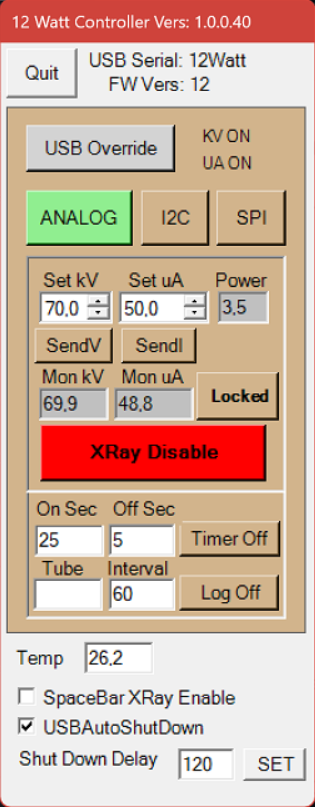
\includegraphics[width=\textwidth]{pictures/12WattController_70kV_10uA.png}
            \caption[Set point of \qty{70}{kV} and \qty{50}{\micro\ampere}]{Set point of \qty{70}{kV} and \qty{50}{\micro\ampere}.}%
            \label{subfig:12WattController 70kV}
        \end{subfigure}
        \caption[XRS GUI tool running on Windows]{XRS GUI tool running on Windows. (a) the filament current maxes out at \(\approx \qty{1100}{\micro\ampere}\). (b) a maximum acceleration voltage of \(\approx\qty{70}{\kilo\volt}\). In any case, the device does not allow exceeding a maximum power of \qty{12}{\watt}.}%
        \label{fig:12WattController 10kV and 70kV}
    \end{figure}
    % \newpage
    % ===================================================================================